\documentclass[11pt]{article}
\usepackage[margin=1.0in]{geometry}
\usepackage{setspace}
\usepackage{amsmath}
\usepackage{fancyhdr}
\usepackage{mathpartir}
\usepackage{listings}
\usepackage{tikz-qtree,tikz-qtree-compat}
\usepackage{tikz}
\pagestyle{fancy}
\lhead{CS 4610 Written Assignment 6}
\rhead{Zihao Wang (zw2rf)}
\cfoot{\thepage}
\renewcommand{\headrulewidth}{0.4pt}
\renewcommand{\footrulewidth}{0.4pt}
\renewcommand{\thesubsection}{\alph{subsection}.}
\lstset {
	language=C++,
	frame=single,
	numbers=none,
	backgroundcolor=\color{white}
}

\begin{document}
\thispagestyle{empty}
\title{CS 4610 Written Assignment 6}
\author{Zihao Wang (zw2rf)}
\date{\today}
\maketitle
\doublespacing

\section{Consider the rules for the constant propagation algorithm discussed in class}
\begin{enumerate}
\item $C_{in}(x,s) = \# \qquad \Rightarrow \qquad C_{out}(x, s) = \#$
\item $C_{in}(x, x \leftarrow c) \qquad \Rightarrow \qquad C_{out}(x, x \leftarrow c) = c \qquad \text{(c is a constant)}$
\item $C_{out}(x, x \leftarrow f(...)) = *$
\item $E(x) \neq E(y) \qquad \Rightarrow \qquad C_{out}(x, y \leftarrow ...) = C_{in}(x, y \leftarrow ...)$
\item $C_{in}(x,s) = lub\{ C_{out}(x, p ) \mid p \text{ is a predecessor of s} \}$
\end{enumerate}

\subsection{Give a concise English description for each of rules 1-4.}
\begin{enumerate}
\item If the value of $x$ is not reachable before an expression that does not involve $x$, that value is still not reachable after the expression
\item Regardless of the status of the variable $x$, after an expression that assigns constants to a variable, the value of $x$ becomes a constant.
\item Regardless of the status of the variable $x$, after an expression that assigns the value of a function call to $x$, the value of $x$ is unknown. 
\item If the value of $x$ is a constant before an expression that assigns value to $y$, the value of $x$ remains at the same constant after it.
\end{enumerate}

\subsection{Give two distinct examples that show some set of predecessor $C_{out}$'s and the resulting $C_{in}$ computation.}
\begin{enumerate}
\item Suppose $C_{out}(x, p_{1}) = \# \quad C_{out}(x,p_{2}) = \# \quad C_{out}(x, p_{3}) = c$, we have $C_{in}(x, s) = c$
\item Suppose $C_{out}(x, p_{i}) = c \quad C_{out}(x, p_{j}) = d \text{ and } c \neq d$, we have $C_{in}(x, s) = *$
\end{enumerate}

\subsection{Briefly explain why the algorithm is guaranteed to terminate.}
At the beginning of the algorithm, every value of a variable $x$ is assigned to $\#$. In this algorithm, each variable changes at most twice ($\# \rightarrow c \text{ and } c \rightarrow *$). Since there are finite number of changes, the algorithm is guaranteed to terminate.  

\subsection{Why is it safe to assume that the evaluation of e does not change the value of $x$}
For an assignment to $y$, the only change made is the value of $y$. As for the expression $e$ on the right hand size, single assignment ensures that the value of $x$ does not change.

\setcounter{subsection}{0}

\section{Consider the fragment of intermediate code}

\subsection{Divide this code into basic blocks.}
\begin{lstlisting}
M0: START 
    if a = 2 goto L3
\end{lstlisting}
\begin{lstlisting}
L0: b := 2
\end{lstlisting}
\begin{lstlisting}
L1: d := a/ 2
    c := a % b
    if c = 0 goto L2
\end{lstlisting}
\begin{lstlisting}
M1: if b >= d goto L3
\end{lstlisting}
\begin{lstlisting}
M2: b := b + 1
    goto L1
\end{lstlisting}
\begin{lstlisting}
L2: a := a + 1
    goto L0
\end{lstlisting}
\begin{lstlisting}
L3: END
\end{lstlisting}

\subsection{Draw a control-flow graph for this program}
\subsection{Annotate your control-flow graph with the set of variables that are live before and after each statement. Assume that only $a$ is live at the entry to $L3$.}


\begin{center}
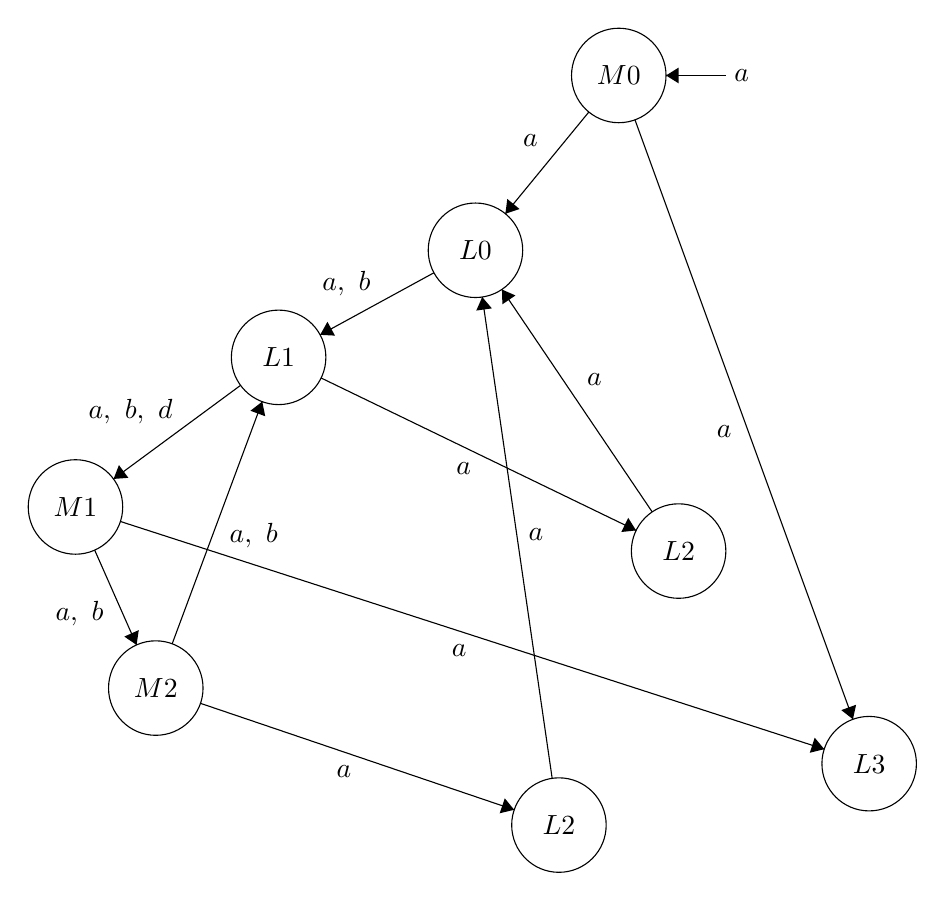
\begin{tikzpicture}[scale=0.2]
\tikzstyle{every node}+=[inner sep=0pt]
\draw [black] (50.4,-7.2) circle (3);
\draw (50.4,-7.2) node {$M0$};
\draw [black] (41.3,-18.3) circle (3);
\draw (41.3,-18.3) node {$L0$};
\draw [black] (66.3,-50.9) circle (3);
\draw (66.3,-50.9) node {$L3$};
\draw [black] (28.8,-25.1) circle (3);
\draw (28.8,-25.1) node {$L1$};
\draw [black] (15.9,-34.6) circle (3);
\draw (15.9,-34.6) node {$M1$};
\draw [black] (54.2,-37.4) circle (3);
\draw (54.2,-37.4) node {$L2$};
\draw [black] (21,-46.1) circle (3);
\draw (21,-46.1) node {$M2$};
\draw [black] (46.6,-54.8) circle (3);
\draw (46.6,-54.8) node {$L2$};
\draw [black] (48.5,-9.52) -- (43.2,-15.98);
\fill [black] (43.2,-15.98) -- (44.1,-15.68) -- (43.32,-15.04);
\draw (45.29,-11.32) node [left] {$a$};
\draw [black] (51.43,-10.02) -- (65.27,-48.08);
\fill [black] (65.27,-48.08) -- (65.47,-47.16) -- (64.53,-47.5);
\draw (57.59,-29.84) node [left] {$a$};
\draw [black] (38.66,-19.73) -- (31.44,-23.67);
\fill [black] (31.44,-23.67) -- (32.38,-23.72) -- (31.9,-22.84);
\draw (33.11,-21.2) node [above] {$a,\mbox{ }b$};
\draw [black] (26.38,-26.88) -- (18.32,-32.82);
\fill [black] (18.32,-32.82) -- (19.26,-32.75) -- (18.66,-31.94);
\draw (19.4,-29.35) node [above] {$a,\mbox{ }b,\mbox{ }d$};
\draw [black] (31.5,-26.41) -- (51.5,-36.09);
\fill [black] (51.5,-36.09) -- (51,-35.29) -- (50.56,-36.19);
\draw (40.56,-31.76) node [below] {$a$};
\draw [black] (17.12,-37.34) -- (19.78,-43.36);
\fill [black] (19.78,-43.36) -- (19.92,-42.42) -- (19,-42.83);
\draw (17.72,-41.34) node [left] {$a,\mbox{ }b$};
\draw [black] (18.75,-35.52) -- (63.45,-49.98);
\fill [black] (63.45,-49.98) -- (62.84,-49.25) -- (62.53,-50.21);
\draw (40.27,-43.29) node [below] {$a$};
\draw [black] (22.04,-43.29) -- (27.76,-27.91);
\fill [black] (27.76,-27.91) -- (27.01,-28.49) -- (27.95,-28.84);
\draw (25.66,-36.41) node [right] {$a,\mbox{ }b$};
\draw [black] (23.84,-47.07) -- (43.76,-53.83);
\fill [black] (43.76,-53.83) -- (43.16,-53.1) -- (42.84,-54.05);
\draw (32.95,-50.98) node [below] {$a$};
\draw [black] (46.17,-51.83) -- (41.73,-21.27);
\fill [black] (41.73,-21.27) -- (41.35,-22.13) -- (42.34,-21.99);
\draw (44.64,-36.37) node [right] {$a$};
\draw [black] (52.52,-34.91) -- (42.98,-20.79);
\fill [black] (42.98,-20.79) -- (43.01,-21.73) -- (43.84,-21.17);
\draw (48.36,-26.51) node [right] {$a$};
\draw [black] (57.2,-7.2) -- (53.4,-7.2);
\draw (57.7,-7.2) node [right] {$a$};
\fill [black] (53.4,-7.2) -- (54.2,-7.7) -- (54.2,-6.7);
\end{tikzpicture}
\end{center}

\subsection{Describe concisely what this program does if the value of $a$ is the only output.}
This program returns the smallest prime number that is no smaller than the input $a$.

\end{document}